\documentclass[10pt,letterpaper]{article}
\usepackage[margin=0.85in]{geometry}
\usepackage[T1]{fontenc}
\usepackage{lmodern,microtype,amsmath,amssymb,booktabs,array,tabularx}
\usepackage{graphicx,xcolor,tikz,pgfplots,caption,subcaption}
\usepackage{adjustbox}
\usepackage[numbers,sort&compress]{natbib}
\usepackage{hyperref}
\usepackage{xurl}
\usepackage{enumitem}
\usetikzlibrary{arrows.meta,positioning,fit,backgrounds}
\usepgfplotslibrary{groupplots}
\pgfplotsset{compat=1.18}
\definecolor{eviblue}{HTML}{1261A0}
\definecolor{prefixorange}{HTML}{CB6B28}
\definecolor{topgreen}{HTML}{327A56}
\hypersetup{colorlinks=true,linkcolor=eviblue,citecolor=eviblue,urlcolor=eviblue,
pdftitle={EviCastKV: PrefixKV Results and Prof. Fox Review Experiments},
pdfauthor={MosaicKV Project},pdfsubject={Artifact-derived experimental report}}
\setlist{itemsep=2pt,topsep=3pt}
\setlength{\emergencystretch}{2em}
\newcommand{\Evi}{EviCastKV}
\newcommand{\MiB}{\,\mathrm{MiB}}
\newcommand{\resulttable}[2]{\begin{center}\small\begin{adjustbox}{max width=#1}\input{generated/#2}\end{adjustbox}\end{center}}
\newcommand{\takeaway}[1]{\par\smallskip\noindent\textbf{Takeaway.} #1\par\smallskip}
\title{\textbf{EviCastKV / MosaicKV: Verified Strengths, PrefixKV Results,\\
and the Prof. Fox Review Experiments}}
\author{Artifact-derived experimental report}
\date{Updated October 30, 2026}

\begin{document}
\maketitle
\begin{abstract}
This report consolidates measured evidence for \Evi, the paper name for
MosaicKV. It emphasizes three supported strengths: favorable initial-cache
and reference-output quality trade-offs in the completed PrefixKV campaign;
higher captioning scores than the local VL-Cache reimplementation at several
shared physical budgets; and a newly verified execution optimization that
reduces exact-tier construction time without changing selected cache entries
or model outputs. These findings have different evidential scopes. The
PrefixKV native-policy comparison is not byte-matched; its initial-memory
advantage does not persist through long append-only generation. The
Prof. Fox routing, coverage, and output-guard studies are development evidence,
not independent confirmation. One earlier engineering result is exact:
on a consumed 120~MiB input, tier construction decreased from 8.604 to
1.333~seconds, with unchanged tokens, logits, positions, and physical storage.
The latest lossless history diagnostic reduces final storage by approximately
14\% and observed decode-owned peak by approximately 13\% on two consumed
LLaVA inputs, preserving all 128 original logits bitwise. Reconstruction is
slower than ordinary K/V history; a direct constructor recovers about 4\%
of source-path decode time at unchanged bytes. These are representation
results, not independent answer-quality or whole-request peak evidence.
The report includes favorable and unfavorable observations, separates
perplexity, ROUGE-L, and CIDEr, and does not claim a general equal-quality
memory or serving-latency advantage.
\end{abstract}
\tableofcontents

\section{Executive findings and claim boundaries}
\label{sec:summary}
\Evi{} and MosaicKV denote the \emph{same system}. Historical artifacts keep
the identifier \texttt{mosaickv\_exact}; they must not be counted as results
from two independent algorithms. All reported \Evi{} performance here concerns
the exact-selection path. Prototype merging and residual repair are not
validated by these measurements.

\paragraph{Where the evidence is favorable.}
\begin{enumerate}
\item \textbf{Native-policy PrefixKV comparison.} On 1,000 descriptions,
\Evi{} achieves 71.09 FullKV-reference ROUGE-L points versus 63.42 for the
faithful local PrefixKV path; on 218 paper-style MM-Vet examples, the values
are 79.03 versus 64.97. Initial mean cache is approximately 103 rather than
150~MiB. These are useful operating points, \emph{not a byte-matched result}.
\item \textbf{Strict shared-byte quality evidence.} At 40~MiB initial cache,
the completed PrefixKV campaign holds physical initial, final, and peak
storage fixed across compressed methods. \Evi{} strongly exceeds the
byte-rescaled, append-only PrefixKV adaptation in reference ROUGE-L, while
remaining close to Prompt Top-K. The adaptation label is essential: its
large degradation is not evidence that the original PrefixKV paper is wrong.
\item \textbf{VL-Cache context.} In the separate historical 256-image COCO
study, \Evi{} exceeds \path{vl_cache_reimpl} at shared 10, 20, and 40~MiB
points in the stored paired analyses. The 80~MiB contrast is unresolved.
This larger result is kept distinct from the review's smaller cohorts.
\item \textbf{A verified systems improvement.} Lazy validated exact-tier
views remove hundreds of thousands of unnecessary host tensor objects.
At 120~MiB, profiled \Evi{} construction improves by 84.5\%; compatible
Prompt Top-K construction benefits from the same implementation.
\item \textbf{Lossless history engineering.} The latest two-input diagnostic
reduces final/observed decode-owned peak storage at unchanged original K/V
and outputs. Section~\ref{sec:historyengineering} separates its memory benefit
and recomputation cost from benchmark evidence.
\end{enumerate}

\paragraph{What these findings do not establish.}
They do not establish that \Evi{} is at least 30\% smaller at the same
quality than the strongest eligible competitor, or that it is generally
faster than PrefixKV, or that opportunity routing and demand coverage are
independently beneficial. Initial savings, full-lifetime savings,
same-budget quality, and representation correctness are different claims.
The latest development gates remain negative; fresh evaluation and larger
campaigns remain blocked.

\section{Evidence organization and experimental controls}
\label{sec:setup}
\subsection{Separate comparison lanes}
Table~\ref{tab:evidence} distinguishes completed large evidence from small
development studies and execution diagnostics. Sample counts cannot be
added across studies that reuse identities.

\begin{table}[htbp]
\centering\small
\caption{Evidence map. R denotes a local reimplementation, not official code.}
\label{tab:evidence}
\begin{tabularx}{\linewidth}{p{0.21\linewidth}p{0.18\linewidth}X}
\toprule
Study & Unique examples & Scope and principal metric\\\midrule
Completed PrefixKV & 1,000 + 218 & Native-policy BF16 and separate shared-byte FP16; corpus PPL and reference ROUGE-L.\\
Intermediate PrefixKV & 32 per task & 80/120/160~MiB development curves; same metric definitions.\\
Historical COCO & 256 images & 10/20/40/80~MiB matched physical budgets; corpus CIDEr.\\
Historical MileBench E6 & 192 examples & Four subtasks, 48 each; separate Accuracy/ROUGE-L; not fresh confirmation.\\
Fox opportunity/coverage & 64 images, reused & Two routing studies over the \emph{same} 64 images; 1,664 request observations, not 128 independent inputs.\\
Fox output guard & 32 images & 288 development requests; CIDEr and descriptive timing.\\
Compact representation & Two consumed inputs & Seven reference/candidate pairs; numerical equality, bytes, and synchronized phase timing.\\
Lossless history engineering & Two consumed inputs, reused & Six paths, two 12-worker comparisons; 128-token bitwise preservation and within-path timing, not new benchmark evidence.\\
\bottomrule
\end{tabularx}
\end{table}

The PrefixKV lane uses \nolinkurl{llava-hf/llava-1.5-7b-hf}, revision
\nolinkurl{b234b804b114d9e37bb655e11cbbb5f5e971b7a9}, on the materialized
LLaVA-Description and paper-style MM-Vet routes. Its pinned upstream
PrefixKV revision is \nolinkurl{597f1ab032704951550f93bcc8a23f1454b80aa4}.
The paper-native campaign uses BF16; the unified byte-capped campaign uses
FP16 and a separate FullKV reference. They are never pooled.

The review COCO lane uses \nolinkurl{llava-hf/llava-v1.6-mistral-7b-hf}, revision
\nolinkurl{2424fdd47412fccc66d91719126b420e9fbd7065}, FP16, Hugging Face
(HF) eager attention. COCO Caption is pinned at revision
\nolinkurl{c3213b54e173ae86517d481de17f31439d6f8c72}. These model families
are not interchangeable experimental repetitions \citep{liu2024improved}.

Within each matched-budget lane, prompts, samples, media, processor,
tokenization, model revision, precision, generation schedule, backend,
mandatory policy, and physical accounting are held fixed. Append-only
generation emits 1,024 tokens in the PrefixKV campaign and 64 in the
review COCO study, with 1,023 and 63 cache-appending forward steps,
respectively. End-of-sequence handling follows each frozen protocol; the
review COCO schedule executes all 64 steps and decodes quality text at the
first terminal token. FullKV is a quality reference, not a compressed-method
latency competitor.

The common environment records Python 3.11.15, PyTorch 2.8.0, Transformers
4.55.2, lmms-eval 0.7.2, and pycocoevalcap 1.2. GPU diagnostics use one
A100 and 12 CPUs per worker. Exact producer revisions, configuration
hashes, model/dataset bindings, software records, and source artifact hashes
are retained in \texttt{provenance.json} and the referenced run manifests.
Installed serving frameworks do not imply that these HF rows execute through
vLLM or SGLang.

\subsection{Metric definitions}
\paragraph{Corpus perplexity (PPL; lower is better).}
For teacher-forced negative log likelihood (NLL) $\ell_i$ over $n_i$
evaluated target tokens,
\begin{equation}
\operatorname{PPL}=\exp\left(\frac{\sum_i\ell_i}{\sum_i n_i}\right).
\end{equation}
Neither per-example PPL nor shard PPL is averaged. The complete campaign
contains 138,905 evaluated target tokens per Description arm and 20,949
per MM-Vet arm. Target masks and token counts belong to the metric phase,
not the separate fixed-length generated answer schedule.

\paragraph{FullKV-reference ROUGE-L (higher is better).}
For generated string $y$ and the frozen FullKV output $r$, let
$L=\operatorname{LCS}(y,r)$ be their longest common subsequence under the
declared tokenizer. The F1 form combines $L/|y|$ and $L/|r|$; the report
shows $100\times\mathrm{F1}$ \citep{lin2004rouge}. This measures reference
output similarity, not factual accuracy against human annotations.
FullKV's score of 100 is constructed by self-reference. The paper-style
MM-Vet route here is \emph{not} the standard judge-based MM-Vet answer score.

\paragraph{CIDEr (higher is better).}
COCO Caption uses the pinned consensus-based corpus evaluator
\citep{lin2014coco,vedantam2015cider}. Corpus document frequencies and
the reducer must be recomputed in each paired bootstrap draw. Shard CIDEr
scores are never averaged. The latest reducer verification reports maximum
absolute difference $8.53\times10^{-14}$ on nine actual-cohort draws;
this validates the reducer algebra, not model numerical parity.

\paragraph{Intervals and multiplicity.}
We reuse the stored 10,000-replicate paired analyses; this writing task
does not rerun inference or choose favorable new contrasts. Historical
PrefixKV intervals are labeled ordinary 95\% intervals. The intermediate
same-budget family has 24 contrasts, its cross-budget family has 16, and
the latest COCO guard family has six, with their stored simultaneous
intervals reported separately. An interval crossing zero is inconclusive,
not proof of equivalence. CIDEr, ROUGE-L, PPL, and MileBench Accuracy are
never combined into an aggregate quality score.

\subsection{Three memory boundaries}
\begin{equation}
M_{\mathrm{init}},\qquad M_{\mathrm{final}},\qquad
M_{\mathrm{peak}}=\max_t M_{\mathrm{live}}(t).
\end{equation}
Memory is measured from physical K/V backing allocations, including padding
and preallocation; $1~\mathrm{MiB}=2^{20}$ bytes. It excludes model weights
and is not total GPU memory. Selected view-payload bytes alone are not a
substitute for physical storage. In a dense append-only layout,
\begin{equation}
M_{\mathrm{final}}=M_{\mathrm{init}}+\Delta M_{\mathrm{decode}},\qquad
\rho_{\mathrm{final}}=1-
\frac{M^{E}_{\mathrm{init}}+\Delta M^{E}_{\mathrm{decode}}}
{M^{B}_{\mathrm{init}}+\Delta M^{B}_{\mathrm{decode}}}.
\end{equation}
Equal initial caps do not automatically imply equal final/peak storage if
maintenance policies differ. The shared-byte exports explicitly check all
three boundaries per sample. Unequal-budget operating points may describe
a frontier, but are not called byte-matched.

\section{PrefixKV: completed large-scale evidence}
\label{sec:prefix}
PrefixKV adapts layer-wise prefix retention \citep{wang2025prefixkv}. The
completed campaign contains 8,526 method--sample rows over 1,218 unique
examples, seven arms per example, and no recorded failures or duplicates.
The native and common-byte lanes have distinct FullKV references and
different decoding semantics. All numbers below are locally measured;
no external paper-reported scores are placed beside them as if measured
in the same execution.

\subsection{Native-policy lane: favorable initial memory and reference quality}
\begin{table}[htbp]
\caption{Completed native-policy campaign: BF16, registered nominal
retention 0.5, 1,000 descriptions and 218 questions. Memory is mean MiB;
R-L is ROUGE-L $\times100$. Policies and realized budgets differ, so this
table is \textbf{not byte-matched}. FullKV latency is intentionally omitted.}
\label{tab:prefixnative}
\resulttable{\linewidth}{prefix_paper_native}
\end{table}

On descriptions, \Evi{} lowers PPL from PrefixKV's 3.0889 to 2.9620 and
raises reference ROUGE-L by 7.67 points. On MM-Vet, ROUGE-L increases by
14.06 points. The stored paired intervals for both ROUGE-L gains exclude
zero (Table~\ref{tab:prefixci}); the native MM-Vet PPL difference is not
statistically resolved. \Evi{} uses approximately 31\% less initial cache
than native PrefixKV on these operating points.

\paragraph{Why this is a useful, but bounded, strength.}
The \Evi{} policy can retain non-prefix evidence selected from prompt
observations rather than restricting its exact evidence to a layer-wise
prefix. Its retained K/V values are unchanged and keep their original
logical positions. The favorable reference-output trade-off is consistent
with retaining prompt-relevant evidence at lower initial storage. However,
selection policy, realized capacity, and decode maintenance all differ in
this lane; the experiment does not isolate a causal selection advantage.

\paragraph{The lifetime trade-off cannot be hidden.}
Native PrefixKV continues profile-based eviction during decoding, whereas
the tested \Evi{} path appends history. Consequently, native PrefixKV ends
near 406--408~MiB while \Evi{} ends near 614--615~MiB. \Evi{} also takes
approximately 64 rather than 53 seconds per request. Thus these native
points support better measured reference quality and lower \emph{initial}
cache, not smaller lifetime cache or lower latency.

\begin{figure}[htbp]
\centering
\begin{tikzpicture}
\begin{groupplot}[group style={group size=2 by 1,horizontal sep=1.25cm},
width=0.46\linewidth,height=5.0cm,ylabel={Mean live KV (MiB)},
xtick={1,2,3},xticklabels={Initial,Final,Peak},ymin=0,ymax=700,
grid=major,legend style={font=\scriptsize,at={(0.03,0.97)},anchor=north west}]
\nextgroupplot[title={1,000 descriptions}]
\addplot+[thick,color=prefixorange,mark=square*] table[x=boundary,y=mib] {generated/native_llava_description_prefix.dat};
\addlegendentry{PrefixKV (R)}
\addplot+[thick,color=eviblue,mark=*] table[x=boundary,y=mib] {generated/native_llava_description_evicast.dat};
\addlegendentry{EviCastKV exact}
\nextgroupplot[title={218 MM-Vet questions}]
\addplot+[thick,color=prefixorange,mark=square*] table[x=boundary,y=mib] {generated/native_mmvet_prefixkv_prefix.dat};
\addplot+[thick,color=eviblue,mark=*] table[x=boundary,y=mib] {generated/native_mmvet_prefixkv_evicast.dat};
\end{groupplot}
\end{tikzpicture}
\caption{Native-policy memory boundaries. Connecting lines only identify
boundaries, not intermediate time measurements. The initial advantage
reverses during generation because maintenance policies differ.}
\label{fig:boundaries}
\end{figure}

\subsection{Shared 40 MiB lane: strict equal-storage comparison}
\begin{table}[htbp]
\caption{Completed FP16 shared-byte lane. Every compressed method has
40~MiB initial and 551.5~MiB final/peak storage per example. PrefixKV (R)
here is a byte-rescaled, append-only adaptation, not the original native
maintenance policy.}
\label{tab:prefixshared}
\resulttable{\linewidth}{prefix_shared_byte_40mib}
\end{table}

At exactly matched physical storage, \Evi{} achieves 63.09 and 72.71
reference ROUGE-L points, versus 13.99 and 13.52 for the transferred
PrefixKV adaptation. This confirms robustness of the tested \Evi{} path
in this unified runtime, \emph{not intrinsic inferiority of native PrefixKV}.
The much stronger simple comparator is Prompt Top-K: it obtains 63.20
and 72.62 points. The differences between \Evi{} and Top-K are small and
unresolved in ROUGE-L; Description PPL is slightly worse for \Evi.
The original PrefixKV native fidelity evidence must therefore remain
separate from this low-budget adaptation.

\begin{table}[htbp]
\caption{\Evi{} minus PrefixKV: aggregate point differences and stored
ordinary paired 95\% intervals, 10,000 replicates. PPL favors negative;
R-L favors positive. The stored interval artifact is preserved without
claiming family-wise correction. Small discrepancies between its stored
bootstrap center and the aggregate point difference are not silently
replaced; only aggregate differences and interval endpoints are shown.}
\label{tab:prefixci}
\resulttable{\linewidth}{prefix_intervals}
\end{table}

\takeaway{The large campaign supports a favorable native-policy
initial-cache/reference-quality trade-off and strong quality against a
specific common-byte PrefixKV adaptation. It does not establish universal
PrefixKV dominance, lower lifetime storage, or improvement over Top-K.}

\section{PrefixKV intermediate-budget development follow-up}
\label{sec:intermediate}
The separately versioned 32-example-per-task follow-up compares the same
three compressed methods at 80, 120, and 160~MiB, with FullKV as a quality
reference. All 640 quality rows complete and byte matching passes. Its
gate nevertheless records \texttt{quality\_memory\_gate=false}; no candidate
is promoted to independent confirmation.

\begin{figure}[htbp]
\centering
\begin{tikzpicture}
\begin{groupplot}[group style={group size=2 by 1,horizontal sep=1.25cm},
width=0.46\linewidth,height=5.3cm,xlabel={Initial physical KV (MiB)},
ylabel={Reference ROUGE-L points},xtick={80,120,160},ymin=0,ymax=90,
grid=major,legend style={font=\scriptsize,at={(0.03,0.04)},anchor=south west}]
\nextgroupplot[title={Description ($n=32$)}]
\addplot+[color=topgreen,mark=triangle*,thick] table[x=cap,y=rouge] {generated/intermediate_llava_description_topk.dat};\addlegendentry{Prompt Top-K}
\addplot+[color=prefixorange,mark=square*,thick] table[x=cap,y=rouge] {generated/intermediate_llava_description_prefix.dat};\addlegendentry{PrefixKV adaptation (R)}
\addplot+[color=eviblue,mark=*,thick] table[x=cap,y=rouge] {generated/intermediate_llava_description_evicast.dat};\addlegendentry{EviCastKV exact}
\nextgroupplot[title={MM-Vet route ($n=32$)}]
\addplot+[color=topgreen,mark=triangle*,thick] table[x=cap,y=rouge] {generated/intermediate_mmvet_prefixkv_topk.dat};
\addplot+[color=prefixorange,mark=square*,thick] table[x=cap,y=rouge] {generated/intermediate_mmvet_prefixkv_prefix.dat};
\addplot+[color=eviblue,mark=*,thick] table[x=cap,y=rouge] {generated/intermediate_mmvet_prefixkv_evicast.dat};
\end{groupplot}
\end{tikzpicture}
\caption{Measured intermediate same-budget development curves. Every
method is evaluated at every displayed cap. Connecting lines are visual
guides, not unmeasured operating points.}
\label{fig:prefixcurves}
\end{figure}

\Evi{} remains close to Top-K and exceeds the PrefixKV adaptation's
ROUGE-L at all three caps, but the complete metric record is important.
At 160~MiB on MM-Vet, the PrefixKV adaptation obtains PPL 5.3237 versus
\Evi's 5.5238, despite lower ROUGE-L (67.69 versus 78.14 points).
PPL predicts annotated target tokens; ROUGE-L compares generated strings
to FullKV. Neither can stand in for the other.

The exploratory 120-versus-160~MiB comparison is \emph{not byte-matched}.
On MM-Vet, \Evi{} improves ROUGE-L against the PrefixKV adaptation under
the stored simultaneous interval, but worsens PPL. On Description, PPL
improves while ROUGE-L preservation is unresolved. The two tasks/metrics
therefore do not jointly pass the registered lower-memory quality gate.
The complete measurements appear in Appendix~\ref{app:intermediate}.

\section{Prof. Fox review: questions, mechanisms, and measured outcomes}
\label{sec:fox}
The review package targets representation correctness, scorer validity,
first-token boundaries, planner cost, graph participation, routing policy,
and confirmation provenance. These checks are not interchangeable: correct
packing does not establish better answers, and a faster internal phase
does not establish end-to-end superiority.

\subsection{What the evaluated exact path actually executes}
\begin{figure}[htbp]
\centering
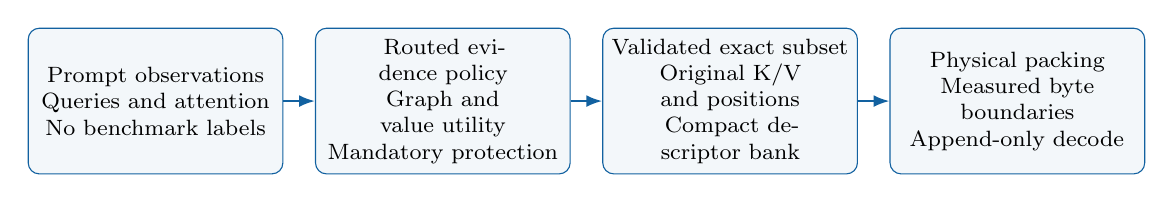
\begin{tikzpicture}[node distance=0.40cm,
box/.style={draw=eviblue,rounded corners,fill=eviblue!5,text width=3.0cm,
minimum height=1.85cm,align=center,font=\footnotesize},
flow/.style={-{Latex[length=2mm]},thick,draw=eviblue}]
\node[box] (obs) {Prompt observations\\Queries and attention\\No benchmark labels};
\node[box,right=of obs] (sel) {Routed evidence policy\\Graph and value utility\\Mandatory protection};
\node[box,right=of sel] (bank) {Validated exact subset\\Original K/V and positions\\Compact descriptor bank};
\node[box,right=of bank] (decode) {Physical packing\\Measured byte boundaries\\Append-only decode};
\draw[flow] (obs)--(sel);\draw[flow] (sel)--(bank);\draw[flow] (bank)--(decode);
\end{tikzpicture}
\caption{Evaluated exact-selection path. Prototype construction and
residual repair are inactive and intentionally absent from this performance
diagram. The representation optimization changes only the third stage and
shared validation work, not the selected subset.}
\label{fig:path}
\end{figure}

\paragraph{Opportunity-aware routing.}
The proposed router seeks heads where a feasible replacement can improve
on the Top-K anchor, rather than simply routing high-entropy heads.
This aims to spend graph work on actionable evidence loss.
\paragraph{Demand-weighted coverage.}
The coverage variant rewards evidence demanded by prompt observations,
rather than uniformly covering every graph node. An important limitation
of the tested implementation is that mapped query heads were averaged;
the record does not establish individual-query-head preservation.
\paragraph{Guarded installation.}
The later output guard checks a proposed route against its anchor and can
roll back a change at unchanged capacity. It tests a prompt-side surrogate,
not the eventual benchmark answer. Rejection is therefore a safety action,
not evidence of semantic improvement.

\subsection{64-image routing and coverage ablations}
\begin{table}[htbp]
\caption{Consumed development data: both studies use the same 64 images.
r256 denotes the 1/256 study; r16 uses its declared 1/16 entropy-routing
comparator, not the original frozen 1/256 policy. CIDEr is recomputed over
the full cohort. All displayed variants are retained, not only winners.}
\label{tab:fox64}
\resulttable{0.85\linewidth}{fox64}
\end{table}

The complete r256 policy reaches 120.89 CIDEr at 40~MiB, versus 120.27
for Top-K and 117.22 for VL-Cache (R). Combining opportunity routing and
demand coverage reaches 121.10, a point gain of 0.83 over Top-K, but its
adjusted interval is $[-1.22,3.21]$. In the r16 study, the combined score
is 120.90 while complete reaches 121.21. Opportunity routing alone lowers
the 40~MiB point estimate in both studies relative to their complete
comparators. These outcomes do not establish mechanism superiority.

The favorable result is narrower: the complete exact policy gives useful
same-capacity CIDEr operating points and its altered policies execute under
controlled physical storage. Increased routing and coverage did not reliably
improve on that policy. The two studies contain 832 observations each but
only 64 unique inputs in total. They remain negative/inconclusive development
studies, not two independent confirmations.

\subsection{32-image installed-output-guard study}
\begin{table}[htbp]
\caption{Latest COCO guard development: 32 images, 288 complete requests.
All compressed methods match initial and final/peak bytes at each cap.
Timing uses zero warmups and one quality request per arm/input; means and
empirical p95 values are descriptive, not repeated microbenchmark evidence.}
\label{tab:fox32}
\resulttable{\linewidth}{fox32}
\end{table}

At 20~MiB, \Evi{} and its guarded variant score 129.56 CIDEr, versus
110.26 for VL-Cache (R). At 40~MiB, the corresponding values are 128.13
and 118.79. The FullKV quality reference is 130.65 CIDEr.
These are favorable point differences at \emph{identical}
physical budgets. The guarded variant matches the complete policy and
Top-K in corpus score; zero observed score difference does not establish
general equivalence outside these consumed inputs.

\begin{table}[htbp]
\caption{Guarded \Evi{} versus VL-Cache (R): CIDEr differences on the
32-image development cohort. The six-contrast family uses simultaneous
coverage 99.1667\% per contrast. The ordinary positive 20~MiB interval
does not survive this registered multiplicity adjustment.}
\label{tab:fox32ci}
\resulttable{0.85\linewidth}{fox32_intervals}
\end{table}

The mean complete-policy request time is 12.50 versus VL-Cache's
16.48 seconds at 20~MiB, and 14.02 versus 18.49 seconds at 40~MiB.
The guarded variant is slightly slower than complete, without a measured
quality gain. These are \emph{descriptive local-runtime observations};
no paired latency confidence bound, production serving kernel advantage,
or general latency win follows from them.

\subsection{Routing audit and why the output guard did not improve quality}
Across the 32 guard requests per budget, the observed route is layer~0,
head~4. The guard accepts changes on five inputs at 20~MiB and two at
40~MiB, changing 166 and 175 selected positions in aggregate; it rolls back
27 and 30 routes, respectively. There are no whole-cache fallbacks in
this audit. Most proposals therefore leave the anchor intact.

The original cohort did not save all entropy scores, so constant routing
alone could not distinguish a genuine winner from an indexing error.
The later consumed-input instrumentation records all 256 scores and
replays the router. On that one COCO input, layer~0/head~4 scores 0.95346,
ahead of head~6 at 0.79800 and head~2 at 0.70036. This validates the
winner for that captured input, not for every historical request.

\takeaway{The complete policy has favorable same-budget point estimates
against the tested VL-Cache port. The new routing/coverage/guard mechanisms
do not yet supply statistically established additional gains, and their
development gates remain negative.}

\section{Larger COCO context: a positive same-budget result}
\label{sec:coco}
The completed historical 256-image COCO experiment provides larger
same-byte evidence than the review diagnostics. It uses the frozen policy,
not a silently substituted review successor. At shared 10, 20, 40, and
80~MiB, \Evi--VL-Cache CIDEr differences are 11.34, 4.35, 3.64, and
0.75, with stored ordinary paired 95\% intervals $[6.55,16.49]$,
$[0.01,8.90]$, $[0.53,7.06]$, and $[-3.09,4.33]$. These intervals are
not presented as fresh, multiplicity-adjusted confirmation.

\begin{figure}[htbp]
\centering
\begin{tikzpicture}
\begin{axis}[width=0.84\linewidth,height=5.8cm,xlabel={Shared initial physical KV (MiB)},
ylabel={Corpus CIDEr},xtick={10,20,40,80},grid=major,
legend style={font=\small,at={(0.97,0.04)},anchor=south east}]
\addplot+[thick,color=eviblue,mark=*] table[x=cap,y=cider] {generated/coco256_evicast.dat};\addlegendentry{EviCastKV exact}
\addplot+[thick,color=topgreen,mark=triangle*] table[x=cap,y=cider] {generated/coco256_topk.dat};\addlegendentry{Prompt Top-K}
\addplot+[thick,color=prefixorange,mark=square*] table[x=cap,y=cider] {generated/coco256_vl.dat};\addlegendentry{VL-Cache (R)}
\end{axis}
\end{tikzpicture}
\caption{Historical 256-image same-budget COCO curves. Every method runs
at every displayed cap. This is quality at matched memory, not evidence of
smaller memory at equal quality.}
\label{fig:coco}
\end{figure}

At 40~MiB, \Evi{} obtains 111.48 CIDEr versus VL-Cache's 107.84, with
mean E2E 16.68 versus 20.75 seconds. Top-K is slightly higher at 111.59
CIDEr. Thus the positive conclusion concerns the measured VL-Cache port,
not all nearest competitors. The complete measured budget table appears
in Appendix~\ref{app:coco}. Historical FP16/BF16 references, cohorts, and
generation protocols must not be interchanged when reusing these rows.

\section{Historical LOOK-M comparison: MileBench E6}
\label{sec:milehistory}
The completed E6 cohort has 192 inputs across ActionPrediction,
ActionSequence, CLEVR-Change, and Spot-the-Diff, 48 per subtask. The first
two contribute Accuracy and the latter two ROUGE-L, 96 applicable examples
per metric family. The pinned MileBench revision is
\nolinkurl{53c7a580}; the immutable artifact records the complete dataset
binding. This uses FP16 LLaVA-1.5, HF eager, and a fixed 64-token schedule.
Every method runs at every listed cap and the exporter verifies all 3,072
rows complete without duplicates/errors and equal per-sample initial/final/peak
storage among compressed methods. These are historical reimplementation
measurements, not official LOOK-M reproduction or fresh confirmation.

\begin{table}[htbp]
\caption{Historical 192-example MileBench E6 curves. Accuracy and ROUGE-L
are separate official-hierarchy metric families, never averaged together.
Mean request times are descriptive, not paired repeated-trial confidence
evidence. FullKV remains a quality reference and is excluded from latency.}
\label{tab:milehistory}
\resulttable{0.95\linewidth}{mile192}
\end{table}

At 40~MiB, \Evi{} measures 22.92\% Accuracy and 15.85 ROUGE-L points,
versus LOOK-M (R)'s 25.00\% and 14.48 points. Its mean request time is
16.71 rather than 34.22 seconds. This is mixed quality, not an all-metric
win. Prompt Top-K measures 22.92\% and 15.88 points at the same storage,
with 18.03 seconds mean time. At 16~MiB, the stored \Evi{} points improve
both metrics against the tight-budget LOOK-M port, but the complete table
also retains its less favorable operating points.

The registered lower-memory quality gate is false: adjusted intervals do
not jointly establish non-inferiority for both metric families. The later
Prof. Fox freshness/source-group limitations and transformed-cache numerical
obligations are not resolved by this historical table. The cohort is not
promoted to independent confirmation, and these results cannot establish
smaller memory at equal quality against the nearest eligible competitor.

\section{Earlier engineering result: compact exact tiers}
\label{sec:compact}
\subsection{Measured bottleneck and safe optimization}
The consumed PrefixKV timing audit runs 20 technical repetitions on one
fixed input per task. Before the compact change, \Evi{} compression averages
15.93 seconds on Description and 16.24 seconds on MM-Vet. Tier construction
alone costs 8.46 and 8.87 seconds. PrefixKV's specialized adaptation bypasses
this generic tier path and takes about 2.5 seconds total compression.
Table~\ref{tab:phases} reports the original measured phases; nested spans
must not be summed twice.

\begin{table}[htbp]
\caption{Pre-optimization compression profile at 120~MiB. Seconds are
means of 20 technical repetitions on one consumed input per task, not
population estimates. Forecast cost is included in total but omitted as
a separate column for space. Trace serialization is excluded.}
\label{tab:phases}
\resulttable{\linewidth}{compression}
\end{table}

The expensive representation creates a separate tiny K and V tensor view
for every retained block, then repeatedly inspects them for validation.
At 120~MiB with one-token blocks, 245,760 retained descriptors imply
491,520 block-view objects. The exact-only HF packer already gathers
directly from original tensors and selected descriptors. Those individual
view objects are unnecessary unless another consumer explicitly requests
one.

The revised \texttt{source\_views} representation stores one frozen alias
per layer/tensor, unchanged ordered descriptors, validated geometry and
payload-byte metadata, and immutable sequence facades. Views are created
and cached on demand. The explicit \texttt{source\_views\_reference}
mode preserves the former eager implementation for comparisons.
This is a shared optimization for \Evi{} and Prompt Top-K, not a
baseline-specific shortcut.

\paragraph{Validation is retained.}
Descriptor provenance, physical bounds, contiguous positions, dtype/device,
duplicate membership, mandatory positions, cross-tier conflicts, and byte
statistics remain checked. Materialized views retain stable object identity,
are revalidated, and participate in cross-tier alias checks. A frozen
source alias prevents source-tensor rebinding from redirecting an existing
exact tier. Selected K/V, logical positions, masks, padding, and physical
capacity are unchanged. Full source aliases are not falsely counted as
compressed backing allocations: the runtime separately measures the packed
cache's actual storage.

\subsection{GPU equivalence and measured phase reduction}
\begin{table}[htbp]
\caption{Synchronized consumed-input reference/compact diagnostic.
Single paired phase timings, \emph{not production-latency estimates}.
Description uses 120~MiB; COCO uses 20/40~MiB. Operations differ where
explicitly named and must not be added.}
\label{tab:compact}
\resulttable{\linewidth}{compact}
\end{table}

Two one-A100 workers execute seven paired comparisons on exactly two
already-consumed inputs. Across all seven pairs, greedy tokens, selected
block catalogs, packed slots/logical positions, and initial/final/peak
physical bytes are identical. Maximum captured logit difference is
\textbf{0.0}. Both model adapters also pass 16-token FullKV generate and
retention-1 reinjection parity, with token agreement 1.0 and zero maximum
logit difference. No per-block views are materialized on the compact
exact-only paths.

The 120~MiB \Evi{} tier-construction phase falls from 8.604 to 1.333
seconds (84.5\% reduction). The shared Top-K descriptor/view phase falls
from 6.806 to 0.512 seconds (92.5\%). Complete-policy COCO tier construction
falls from 1.762 to 0.571 seconds at 20~MiB and from 3.218 to 0.761 seconds
at 40~MiB. Guarded variants show the same qualitative reduction.
The full CPU suite passes 2,107 tests; the additional analysis regression
also passes, as do targeted Ruff and MyPy checks.

\begin{figure}[htbp]
\centering
\begin{tikzpicture}
\begin{axis}[ybar,bar width=18pt,width=0.83\linewidth,height=5.4cm,
ylabel={Profiled tier construction (seconds)},symbolic x coords={1,2,3},
xtick=data,xticklabels={Description 120 MiB,COCO 20 MiB,COCO 40 MiB},
x tick label style={font=\small},ymin=0,ymax=10,grid=major,
legend style={font=\small,at={(0.97,0.96)},anchor=north east}]
\addplot+[fill=prefixorange!60,draw=prefixorange] table[x=x,y=reference] {generated/compact_tier.dat};\addlegendentry{Eager views}
\addplot+[fill=eviblue!60,draw=eviblue] table[x=x,y=compact] {generated/compact_tier.dat};\addlegendentry{Compact views}
\end{axis}
\end{tikzpicture}
\caption{Same consumed inputs and unchanged selected state: a representation
optimization, not a new compression ratio. Single-pair profiling cannot
establish an end-to-end speedup distribution.}
\label{fig:compact}
\end{figure}

The GPU jobs \texttt{22139787\_0} and \texttt{22139787\_1} complete in
6:33 and 2:49; automatic CPU analysis \texttt{22139788} completes in
three seconds with \texttt{passed\_diagnostic\_only}. No new benchmark
labels, fresh samples, or larger campaigns are used. We do not subtract
the saved phase time from old campaign latencies and call that a measured
new end-to-end result.

% Narrative companion to hash-bound export_report.py tables.
\section{Lossless storage and history engineering: October 30 update}
\label{sec:historyengineering}
\subsection{Scope and correctness}
The final engineering source is
\nolinkurl{d8eb51be69c5d6469ba12283f0cf811ba352345c}, local branch
\nolinkurl{evicastkv/storage-transport-20261030}. The sealed CPU suite records
2,631 passing tests, no failures/errors/skips. Both six-path GPU comparisons
complete all 12 workers and pass registered numerical/storage controls.
This is engineering readiness, not independent paper-quality confirmation.

All measurements reuse two consumed inputs: Description
\texttt{000000532947} and MM-Vet-route \texttt{v1\_197}, logical lengths
600/604. They use the pinned LLaVA-1.5 model in Section~\ref{sec:setup},
BF16, HF eager, batch one, one A100 per worker. The fixed 128-token schedule
uses the prefill prediction plus 127 decode forwards without early EOS stop.
Five warmups and 20 timed repetitions randomize paired format order within
each method/input worker. Intervals resample technical pairs, not independent
examples. No new benchmark identities or selection policies are introduced.

The six paths are an all-position lossless control, Prompt Top-K, local
append-only PrefixKV/VL-Cache adaptations, LOOK-M (R), and frozen
\path{mosaickv_exact}. LOOK-M retains its actual merged prompt K/V. The
all-position control retains every source position but encodes storage;
its memory is not ordinary uncompressed FullKV memory. Ordinary FullKV
remains the separate numerical/quality reference, excluded from latency.

\subsection{Mechanism: save a shared source, reconstruct exact K/V}
Source history stores encoded normalized layer inputs, logical maps, rotary
phases, and sparse bit corrections restoring original cached bits. A short
raw K/V tail and an additional normalized-input tail support online sealing.
Sealing commits transactionally only after original-K/V checks pass. Model
projections reconstruct unchanged values and positions. Sharing a projection
source saves history bytes without removing evidence, but costs recomputation.
This is a separately labeled lossless representation experiment, not prototype
merging or residual repair. The direct constructor removes an intermediate
format, reducing projection passes nine to four while retaining three final
original-K/V checks. The same optimization applies to the baseline paths.

\begin{table}[htbp]
\caption{Consumed-input storage in MiB. KV means ordinary lossless K/V
history within the same encoded-prompt path, not FullKV; source means
source-sealed history. Initial bytes are unchanged within each pair. Peak is
observed decode-owned storage, not whole-request HBM peak. These are format
differentials, not byte-matched selector comparisons.}
\label{tab:historystorage}
\resulttable{\linewidth}{history_storage}
\end{table}

For \Evi{}, final bytes fall 109.271 to 93.787~MiB on Description and
109.377 to 93.920~MiB on MM-Vet, approximately 14.2\%/14.1\%. Observed
decode-owned peak falls 119.474 to 103.990~MiB and 119.580 to 104.123~MiB,
approximately 13.0\%/12.9\%. Initial stays 61.543/61.688~MiB. This improves
final/peak storage within the same selection, not initial bytes or selection
quality.

\begin{figure}[htbp]
\centering
\begin{tikzpicture}
\begin{groupplot}[group style={group size=2 by 1,horizontal sep=1.2cm},
width=0.46\linewidth,height=5.0cm,ylabel={Owned storage (MiB)},
xtick={1,2,3},xticklabels={Initial,Final,Decode peak},ymin=0,ymax=130,
grid=major,legend style={font=\scriptsize,at={(0.03,0.97)},anchor=north west}]
\nextgroupplot[title={Consumed Description input}]
\addplot+[thick,color=prefixorange,mark=square*] table[x=boundary,y=ordinary] {generated/history_boundaries_llava_description.dat};
\addlegendentry{Ordinary lossless K/V history}
\addplot+[thick,color=eviblue,mark=*] table[x=boundary,y=source] {generated/history_boundaries_llava_description.dat};
\addlegendentry{Lossless source history}
\nextgroupplot[title={Consumed MM-Vet input},ylabel={}]
\addplot+[thick,color=prefixorange,mark=square*] table[x=boundary,y=ordinary] {generated/history_boundaries_mmvet_prefixkv.dat};
\addplot+[thick,color=eviblue,mark=*] table[x=boundary,y=source] {generated/history_boundaries_mmvet_prefixkv.dat};
\end{groupplot}
\end{tikzpicture}
\caption{EviCastKV format differential at unchanged selected evidence.
Lines identify accounting boundaries, not measurements over time.}
\label{fig:historyboundaries}
\end{figure}

The boundary charges payloads, source packets, corrections, phases, maps,
raw/normalized tails, layer leases, and observed constructor/reconstruction
tensors. It excludes inactive original prefill/captures, weights, attention
activations, internal GEMM workspace, and allocator reserve. Original prefill
can determine whole-request peak, which remains uncertified. Source-slot
capacity is fixed across paths but realized encoded bytes differ: this is
not a new common-physical-byte selection-policy comparison.

\subsection{Latency: constructor improvement within a slower storage path}
\begin{table}[htbp]
\caption{Fixed-schedule decode seconds. Source/KV comes from the K/V versus
source-history study; remaining columns come from a separate reference-source
versus direct-source constructor study. Do not combine medians across studies.
Intervals are ordinary technical-pair 95\% intervals, not population or
multiplicity-adjusted intervals.}
\label{tab:historylatency}
\resulttable{\linewidth}{history_latency}
\end{table}

Reference source history is 29.6--29.7\% slower than ordinary lossless K/V
history for \Evi{} here, roughly 29--36\% slower across compressed paths.
The direct constructor improves on that source-history reference: \Evi{}
p50 changes 11.742 to 11.282 seconds and 11.765 to 11.300 seconds, paired
reductions about 3.9--4.0\%, with identical initial/final/observed-peak bytes.
All ten within-path/input direct/reference upper confidence bounds are below
one. This does not prove no-slower execution against ordinary K/V history.

Timing includes online sealing/reconstruction but excludes original prefill,
selection, and initial prompt construction. Different methods use separate
GPU workers; cross-method medians are not paired latency wins. Earlier
roughly 12\% dual-projection decode and 57\% direct prompt-construction
improvements concern distinct references/phases; do not add their percentages
or subtract them from old end-to-end campaign times.

\subsection{What remains negative}
All 128 logits/tokens remain bitwise unchanged relative to each path's own
original selected/merged-cache transport, not necessarily FullKV. The
original 32-token model-reference outcomes remain different across selectors.

\begin{table}[htbp]
\caption{Consumed-input controls: R-L is model-generated FullKV-reference
ROUGE-L $\times100$, not annotation accuracy, corpus PPL, or standard MM-Vet
judge scoring. Bitwise preservation concerns 128 logits relative to each
path's original transport.}
\label{tab:historyquality}
\resulttable{0.95\linewidth}{history_quality_controls}
\end{table}

Description is a counterexample to universal superiority: the PrefixKV
adaptation has smaller final storage than \Evi{} with tied model-reference
quality. MM-Vet retains a quality deficit relative to FullKV for several
selections, including \Evi{}. The codec preserves, rather than repairs,
these outcomes. Negative quality interventions, short-history feasibility,
and the unpromoted checkpoint latency failure remain preserved. No fresh
campaign follows from the engineering pass alone.

\section{Paper-writing priorities}
\label{sec:writingactions}
\begin{enumerate}
\item Lead with the completed 256-image shared-byte COCO curves and separate
1,000/218 PrefixKV native/shared-byte tables. Retain all points and intervals,
Top-K ties/losses, and native final-memory/latency disadvantages. Do not use
the anomalous byte-rescaled adaptation as original-PrefixKV quality evidence.
\item Separate same-budget quality, equal-quality memory, initial savings,
and lifetime savings. A general ``30\% smaller than the nearest competitor
at preserved quality'' headline is not supported.
\item Put representation results in an engineering subsection/appendix with
the consumed identities, exact boundaries, lossless controls, and slower
ordinary-history comparison. Do not replace benchmark tables with diagnostics.
\item Keep claims limited to exact selection and separately labeled lossless
variants. Prototype/repair, other architectures, and native serving gain no
performance validation from this work.
\item Broader claims require a frozen candidate, certified memory boundary,
and disjoint paired native-metric validation, with common optimizations also
applied to competitors. These remain research requirements, not experiments
launched by this writing update.
\end{enumerate}


\section{Why the favorable results are plausible---and what is not proven}
\label{sec:interpretation}
\paragraph{Evidence placement versus prefix placement.}
The native PrefixKV result is consistent with a prompt-conditioned exact
subset preserving information that a fixed prefix misses. The same-byte
adaptation comparison demonstrates that this local exact path tolerates
that particular transferred-profile regime better. It does not isolate
which evidence source causes the quality gain, and no benchmark answers
may be used to select retained entries.

\paragraph{More routing does not guarantee more useful evidence.}
The review ablations test the intended mechanism directly. Opportunity
routing alone is worse at 40~MiB in both 64-image studies. A graph can
cover more nodes without preserving answer-critical evidence; averaging
query heads can suppress rare demand. The guarded study accepts few
modifications and adds no observed corpus-score gain. These results
limit causal claims about inter-modal graph benefits.

\paragraph{Execution efficiency is a different success.}
The lazy bank removes work that is mathematically unnecessary for the
exact packer. Unlike a quality-oriented policy change, its desired outcome
is exact equivalence, which is directly verified. The same optimization
benefits the shared baseline, so it cannot by itself create an algorithmic
quality advantage or a smaller selected KV cache.

\paragraph{Long generation changes the memory story.}
At 1,024 generated tokens, the shared PrefixKV lane appends 511.5~MiB.
A modest initial-cache saving becomes a small share of final memory.
Native PrefixKV's continued eviction can therefore beat append-only
\Evi{} in final storage despite losing in initial storage or reference
quality. A future lifetime-budget algorithm would be a separately
registered method, not a reinterpretation of these results.

\section{Readiness, limitations, and defensible report language}
\begin{table}[htbp]
\centering\small
\caption{Claim ledger: positive results and remaining boundaries.}
\label{tab:claims}
\begin{tabularx}{\linewidth}{p{0.30\linewidth}X}
\toprule
Claim & Current status\\\midrule
Higher native-policy reference ROUGE-L than PrefixKV (R) & Supported on the completed 1,000/218 cohorts; not matched physical budgets.\\
Lower native-policy initial KV & Supported; final/peak advantage reverses under different maintenance policies.\\
Higher same-byte quality than PrefixKV adaptation & Supported in the measured FP16 adaptation regime; not an intrinsic original-PrefixKV conclusion.\\
Higher same-byte COCO CIDEr than VL-Cache (R) & Supported in several historical points; latest small adjusted guard contrasts remain unresolved.\\
Historical MileBench versus LOOK-M (R) & Tight-budget gains and mixed 40~MiB quality; lower-memory quality gate failed; not fresh confirmation.\\
Opportunity/coverage/guard superiority & Not established; development results preserved as negative/inconclusive.\\
Exact-tier representation acceleration & Verified on two consumed inputs with unchanged tokens, logits, positions, and bytes.\\
Lossless history storage reduction & Verified final/decode-owned-peak savings on two consumed inputs; initial unchanged, ordinary-history path faster.\\
Direct source-history constructor & Same-byte bitwise-preserving paired acceleration; not general end-to-end superiority.\\
General latency win or equal-quality lower lifetime memory & Not established.\\
Fresh MileBench confirmation & Blocked by exhausted/uncertified source-group freshness and numerical restrictions; development-only evidence is not promoted.\\
Boundary-B broad numerical validity & Remains restricted by failed controls in historical diagnostics; exact-cache success does not resolve it.\\
Prototype/repair or native serving advantage & Not validated by the evaluated exact-path evidence.\\
\bottomrule
\end{tabularx}
\end{table}

\paragraph{Suggested positive summary.}
``\Evi{} demonstrates favorable initial-cache/reference-output trade-offs
against the tested PrefixKV implementation and competitive or improved
captioning quality at shared physical budgets. Its exact-cache construction
is now substantially cheaper without changing model outputs. The
experiments also expose limits: native PrefixKV remains faster in the
reported large campaign and retains less final cache, while the new
routing and coverage variants have not established additional quality gains.''

This wording emphasizes measured progress without claiming a universal
winner. All inspected development cohorts remain consumed, no new frozen
quality candidate is asserted, and fresh evaluation or larger execution
remains blocked. MileBench's declared Accuracy and ROUGE-L hierarchy
\citep{song2024milebench}, LOOK-M transformed-cache fidelity
\citep{wan2024lookm}, and the failed COCO boundary-B diagnostics are separate
obligations, not resolved by a PrefixKV or representation pass.

\appendix
\clearpage
\section{Complete intermediate PrefixKV measurements}
\label{app:intermediate}
\begin{table}[htbp]
\caption{All intermediate development points, 32 examples per task and arm.
PrefixKV denotes the byte-rescaled append-only adaptation in this table.
PPL and reference ROUGE-L are intentionally separate columns.}
\resulttable{0.94\linewidth}{prefix_intermediate}
\end{table}
The complete same-budget and cross-budget adjusted interval families are
exported as \path{generated/prefix_same_budget_intervals.csv} and
\path{generated/prefix_cross_budget_intervals.csv}. Keeping all
contrasts prevents selective reporting of only the favorable metric.

\section{Historical COCO measurements at every shared budget}
\label{app:coco}
\begin{table}[htbp]
\caption{All historical 256-image shared-byte points. Final equals peak
in these rows; mean E2E includes compression and is descriptive. The
FullKV quality reference is 111.2424 CIDEr and is not a latency competitor.}
\resulttable{0.92\linewidth}{coco256}
\end{table}

\clearpage
\section{Artifact inventory and reproducibility}
\label{app:artifacts}
This report is a CPU-only export of existing artifacts. No inference,
dataset materialization, label-based selection, or new bootstrap family
was performed. Raw predictions and producer files are unchanged.
The exporter independently checks 8,526 complete PrefixKV rows, expected
task counts, duplicate absence, common sample sets, and per-sample equality
of initial/final/peak shared-lane bytes. It verifies the recorded hashes
for the consumed representation diagnostic and bound review evidence.

The report directory contains \texttt{main.tex}, a locally extracted
\texttt{references.bib}, generated tables and plot data,
\texttt{export\_report.py}, and \texttt{provenance.json}. The provenance
ledger records source artifact SHA-256 values, derived hashes, producer
SHAs, and the fact that this writing task occurs in a pre-existing dirty
user worktree. That does not relabel the source experiments as dirty or
clean; their own immutable manifests determine their execution status.

\begin{description}[style=nextline,font=\normalfont\bfseries]
\item[P1: completed PrefixKV campaign]
\path{/scratch/djy8hg/runs/mosaickv/prefixkv/full-campaign-e4de390-20261019-v6}
\item[P2: intermediate PrefixKV development]
\path{/scratch/djy8hg/runs/mosaickv/prefix-native-intermediate-20261029-v2-retry1}
\item[F1: 64-image review evidence closure]
\path{/scratch/djy8hg/runs/evicastkv/fox-review-20261028-writing-closure-v2-report-retry1}
\item[F2: installed-output-guard development]
\path{/scratch/djy8hg/runs/evicastkv/fox-installed-guard-20261029-v2-retry1}
\item[A1: CPU routing, PrefixKV-boundary, and compression audit]
\path{/scratch/djy8hg/runs/evicastkv/cpu-routing-prefix-audit-20261029-v1}
\item[D1: full-score and tier instrumentation]
\path{/scratch/djy8hg/runs/evicastkv/consumed-routing-tier-diagnostic-20261029-v1}
\item[D2: compact exact-tier equivalence and timing]
\path{/scratch/djy8hg/runs/evicastkv/compact-exact-views-consumed-20261029-v1}
\par Producer: \nolinkurl{7472d7ccf9bb670b6921398cada04f6cfd2a5f85}.
\item[C1: historical 256-image COCO shared-byte curves]
\path{/scratch/djy8hg/runs/mosaickv/coco-shared-32-edb6edf-retry1-20261014/analysis/lower-memory-frontier-21636391}
\item[M1: historical 192-example MileBench E6]
\path{/scratch/djy8hg/runs/mosaickv/milebench-isoquality-e6-fdeca17-20261020/analysis/larger}
\item[E1: final engineering readiness, 2,631 passing CPU tests]
\path{/scratch/djy8hg/runs/evicastkv/storage-engineering-final-readiness-20261030-v1}
\item[E2: ordinary K/V history versus source history]
\path{/scratch/djy8hg/runs/evicastkv/source-history-runtime-final-report-20261030-v1}
\par Producer: \nolinkurl{33bc214fba36b30e51ec23b800fbbf08e786f8d3}.
\item[E3: reference versus direct source-history constructor]
\path{/scratch/djy8hg/runs/evicastkv/source-history-direct-final-report-20261030-v1}
\par Producer: \nolinkurl{d8eb51be69c5d6469ba12283f0cf811ba352345c}.
\end{description}

\bibliographystyle{plainnat}
\bibliography{references}
\end{document}
